\documentclass[border=10pt]{standalone}
\usepackage{pgfplots}
\pgfplotsset{compat=1.18}
\begin{document}
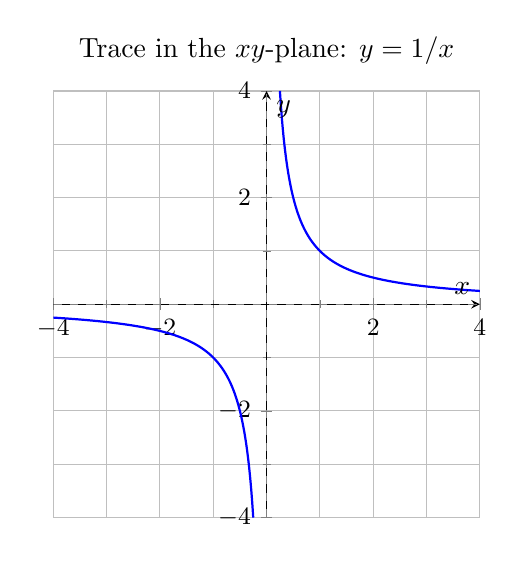
\begin{tikzpicture}
\begin{axis}[
    axis lines=middle,
    xlabel={$x$},
    ylabel={$y$},
    xmin=-4, xmax=4,
    ymin=-4, ymax=4,
    width=8cm, height=7cm,
    grid=both,
    minor tick num=1,
    tick label style={font=\small},
    axis equal image,
    title={Trace in the $xy$-plane: $y=1/x$},
]
\addplot[blue, thick, domain=-4:-0.25, samples=200] {1/x};
\addplot[blue, thick, domain=0.25:4, samples=200] {1/x};
\addplot[dashed, gray, very thin, domain=-4:4, samples=2] {0};
\addplot[dashed, gray, very thin, samples=2] coordinates {(0,-4) (0,4)};
\end{axis}
\end{tikzpicture}
\end{document}